\chapter{Angry Real Analysis that will be eventually omitted}



\section[Baby Rudin]{Baby Rudin Independent Study... I need an A and More}
This is the crux of what is meant to be taught and gained. 

\section{Chapter 1 Baby Rudin}


\newpage

\subsection{Pset 1}


\subsubsection*{Problem 1:} \\ 
If r is rational $(r \neq 0)$ and x is irrational, prove that r+x and rx are irrational. \\ 




This is a proof by contradition: \\


Proof: 
\\
Suppose r is rational and $r=\frac{m}{n}$ where m and n are in the set of integers.   \\
Case 1: 
Assume r+x is rational. \\ 
Let r+ x = $\frac{p}{q}$ where p and q are in the set of relatively prime integers.\\ 
Then $x= \frac{p}{q}-r.$ \\ 
$x=\frac{p}{q}-\frac{m}{n}.$ \\ 
$x= \frac{pn-qm}{qn}.$ \\ 
Thus, x is rational, hence a contradiction. \\
Therefore, r+ x is irrational.  \\ 

Case 2: 
Next, assume rx is rational. 
Then $rx =\frac{p}{q}$ where p and q are in the set of integers. \\ 
Then, $x=\frac{p}{rq}.$ \\ 
So, $x= \frac{p}{\frac{m}{n}q}.$ \\ 
$x=\frac{np}{mq}.$ \\ 
Thus, x is rational, hence a contradiction. 
\\ Therefore, rx is irrational. \\ 


\\
Thus, if r is rational and x is irrational, then r+x and rx are irrational. 

\begin{figure}[h]\begin{center}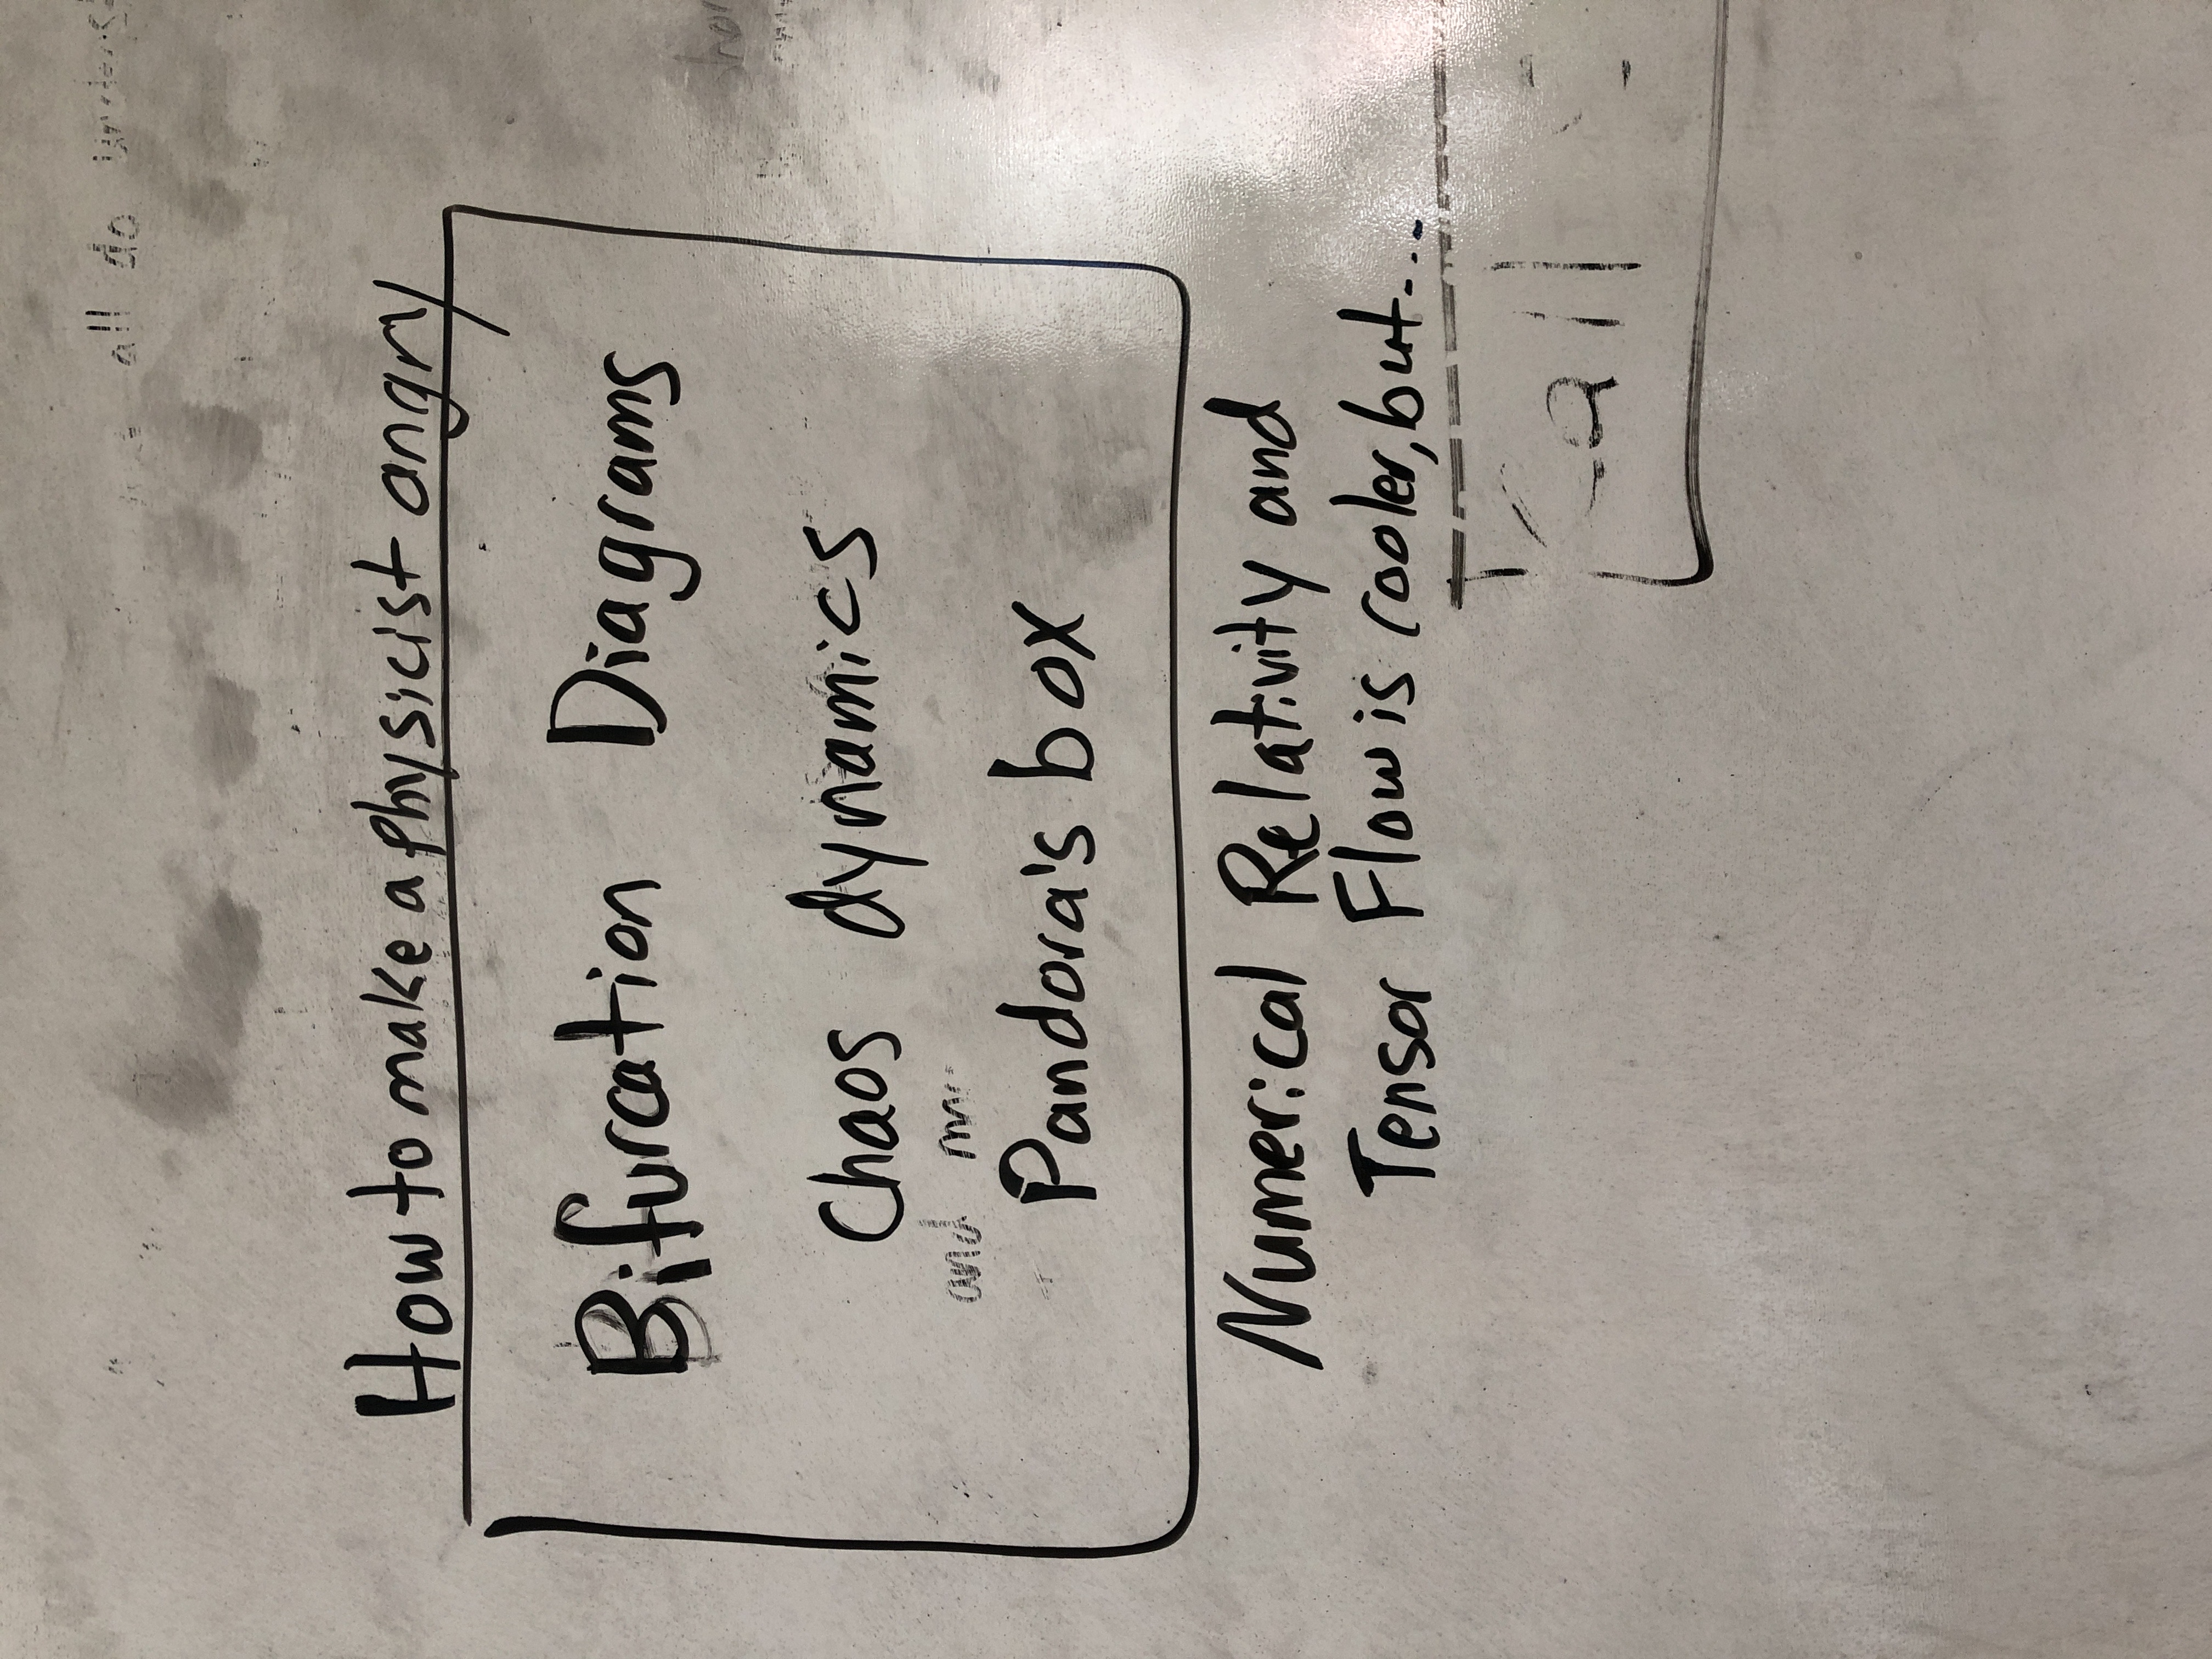
\includegraphics[angle=, origin=c,width=5 in]{Figures/IMG_1052.JPG}
\caption{Placeholder for my proofs} \label{fig:Euler_pic}\end{center}\end{figure} 


\newpage
\subsubsection*{Problem 2:} \\ 
Prove that there is no rational number whose square is 12. \\ 
Proof by contradiction:\\ 
Since $\sqrt{12}=\sqrt{4} \sqrt{3}= 2 \sqrt{3}$,  and from above then $\sqrt{3}$ is irrational. \\ 
Assume that if m and n are integers and have no common factors. \\ 
Since $m^2$ is divisible by 3, then m is divisible by 3. \\  
So $m^2 = 3n^2.$ \\  Let m =3k. \\ 
Then $m^2= 9k^2,$ and we have $3k^2= n^2.$ \\ 
Therefore n is divisible by 3. \\ 
So m and n have no common factor and n is divisible by 3, hence a contradiction.  
\\
Thus, there is no rational number whose square is 12.

\begin{figure}[ht]\begin{center}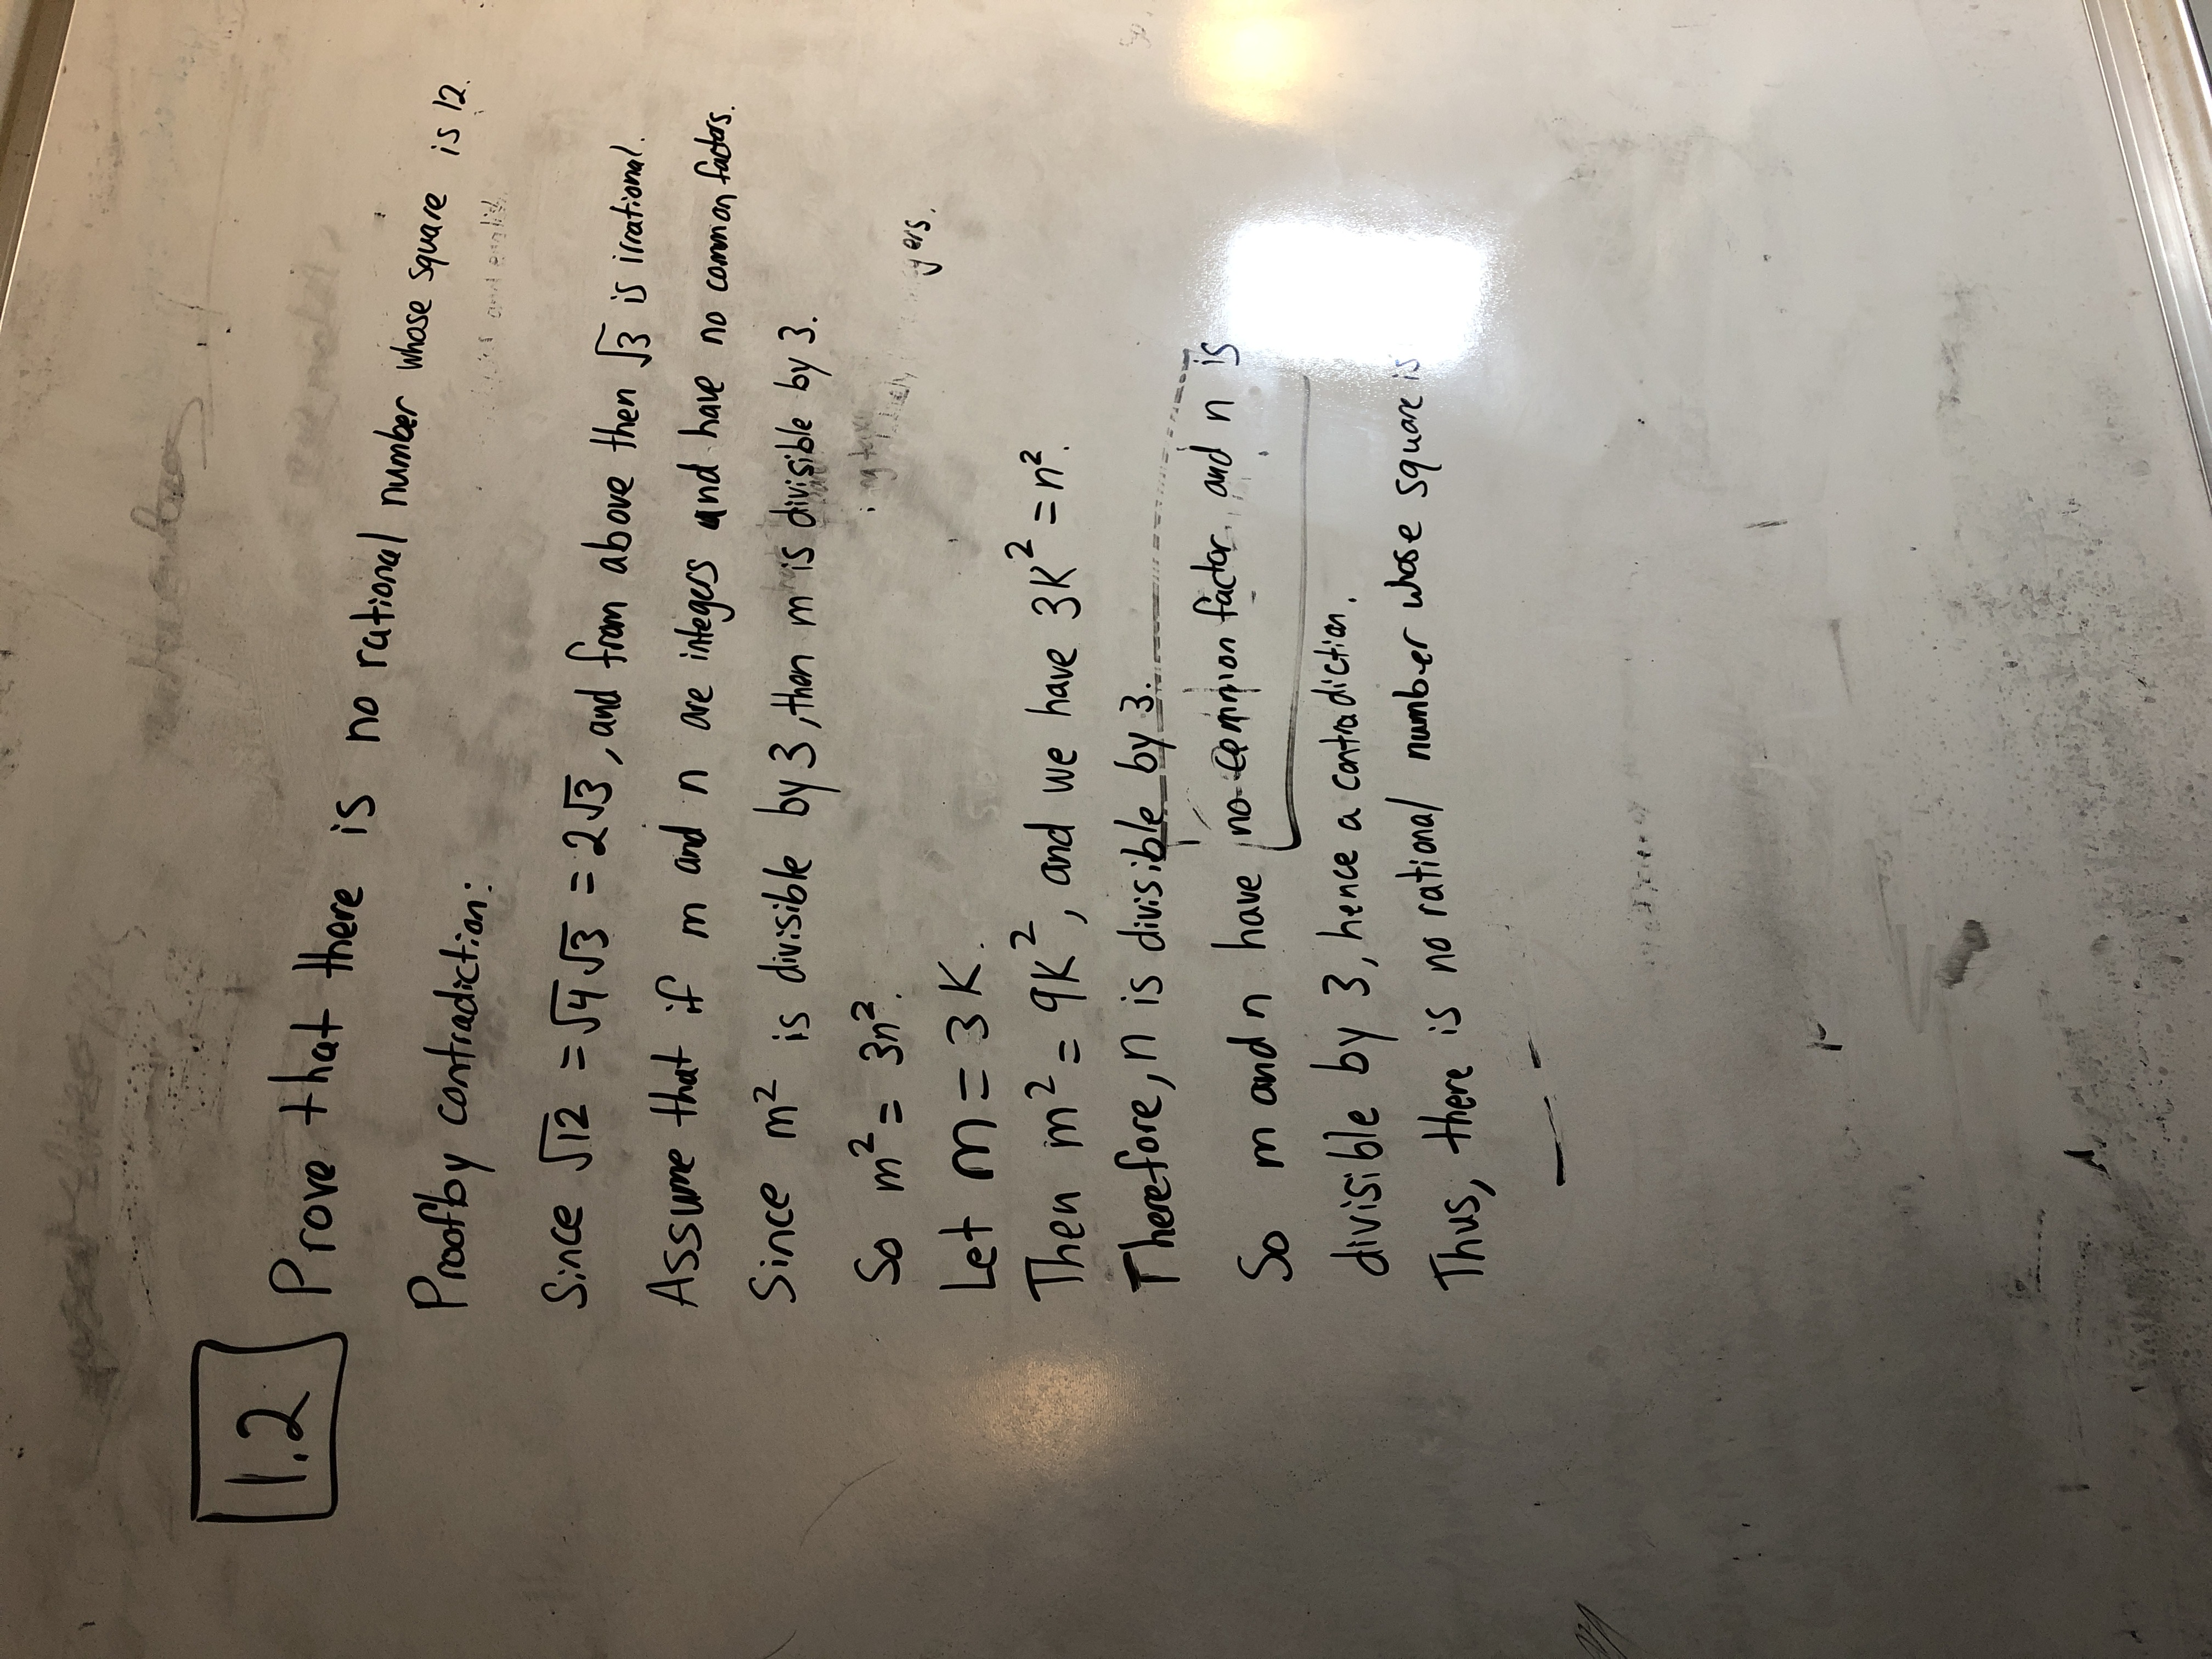
\includegraphics[angle=, origin=c,width=5 in]{Figures/IMG_1077.JPG}
\caption{Placeholder for my proofs} \label{fig:Euler_pic}\end{center}\end{figure} 







\newpage

\section{The First Compilation}

Brain get it out.

\section{Chapter 2 Baby Rudin}

\section{The Second Compilation}



\section{Chapter 3 Baby Rudin}


\section{The Third Compilation}


\section{Chapter 4 Baby Rudin}



\section{Chapter 5 Baby Rudin}


Work work work.




\section{}